\def\VCDate{2015/10/02}\def\VCVersion{(Current)}
\documentclass{article}
\usepackage[screen]{geometry}
\usepackage{ProofPower, graphicx}
\begin{document}
cs118
\begin{GFT}{SML}
\+open TextIO;\\
\+output(stdOut,"Hello from sml\Backslash{}n");\\
\+val x1 = 17;\\
\+val x2 = 3;\\
\+val x3 =1;\\
\+val x4 = 1000;\\
\+x1 + x2 + x3 + x4;\\
\end{GFT}
In a functional language we evaluate expression rather than change the store. Our expected result from adding those 4 values is 1021: \\
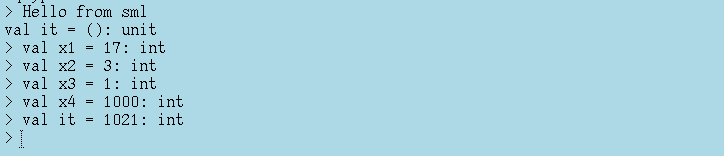
\includegraphics{fig_sml.png}
\clearpage

The following code is a simple C program to display hello
\begin{GFT}{C source code written to file lab.c}
\+\#include <stdio.h>\\
\+int main()\\
\+\{\\
\+  printf("Hello\Backslash{}n");\\
\+  int x1 =17;\\
\+  int x2 = 3;\\
\+  int x3 = 1;\\
\+  int x4 = 1000;\\
\+  x1 += x2;\\
\+  x1 += x3;\\
\+  x1 += x4;\\
\+  printf("The value of x1 is \%d\Backslash{}n",x1);\\
\+  return 0;\\
\+\}\\
\end{GFT}
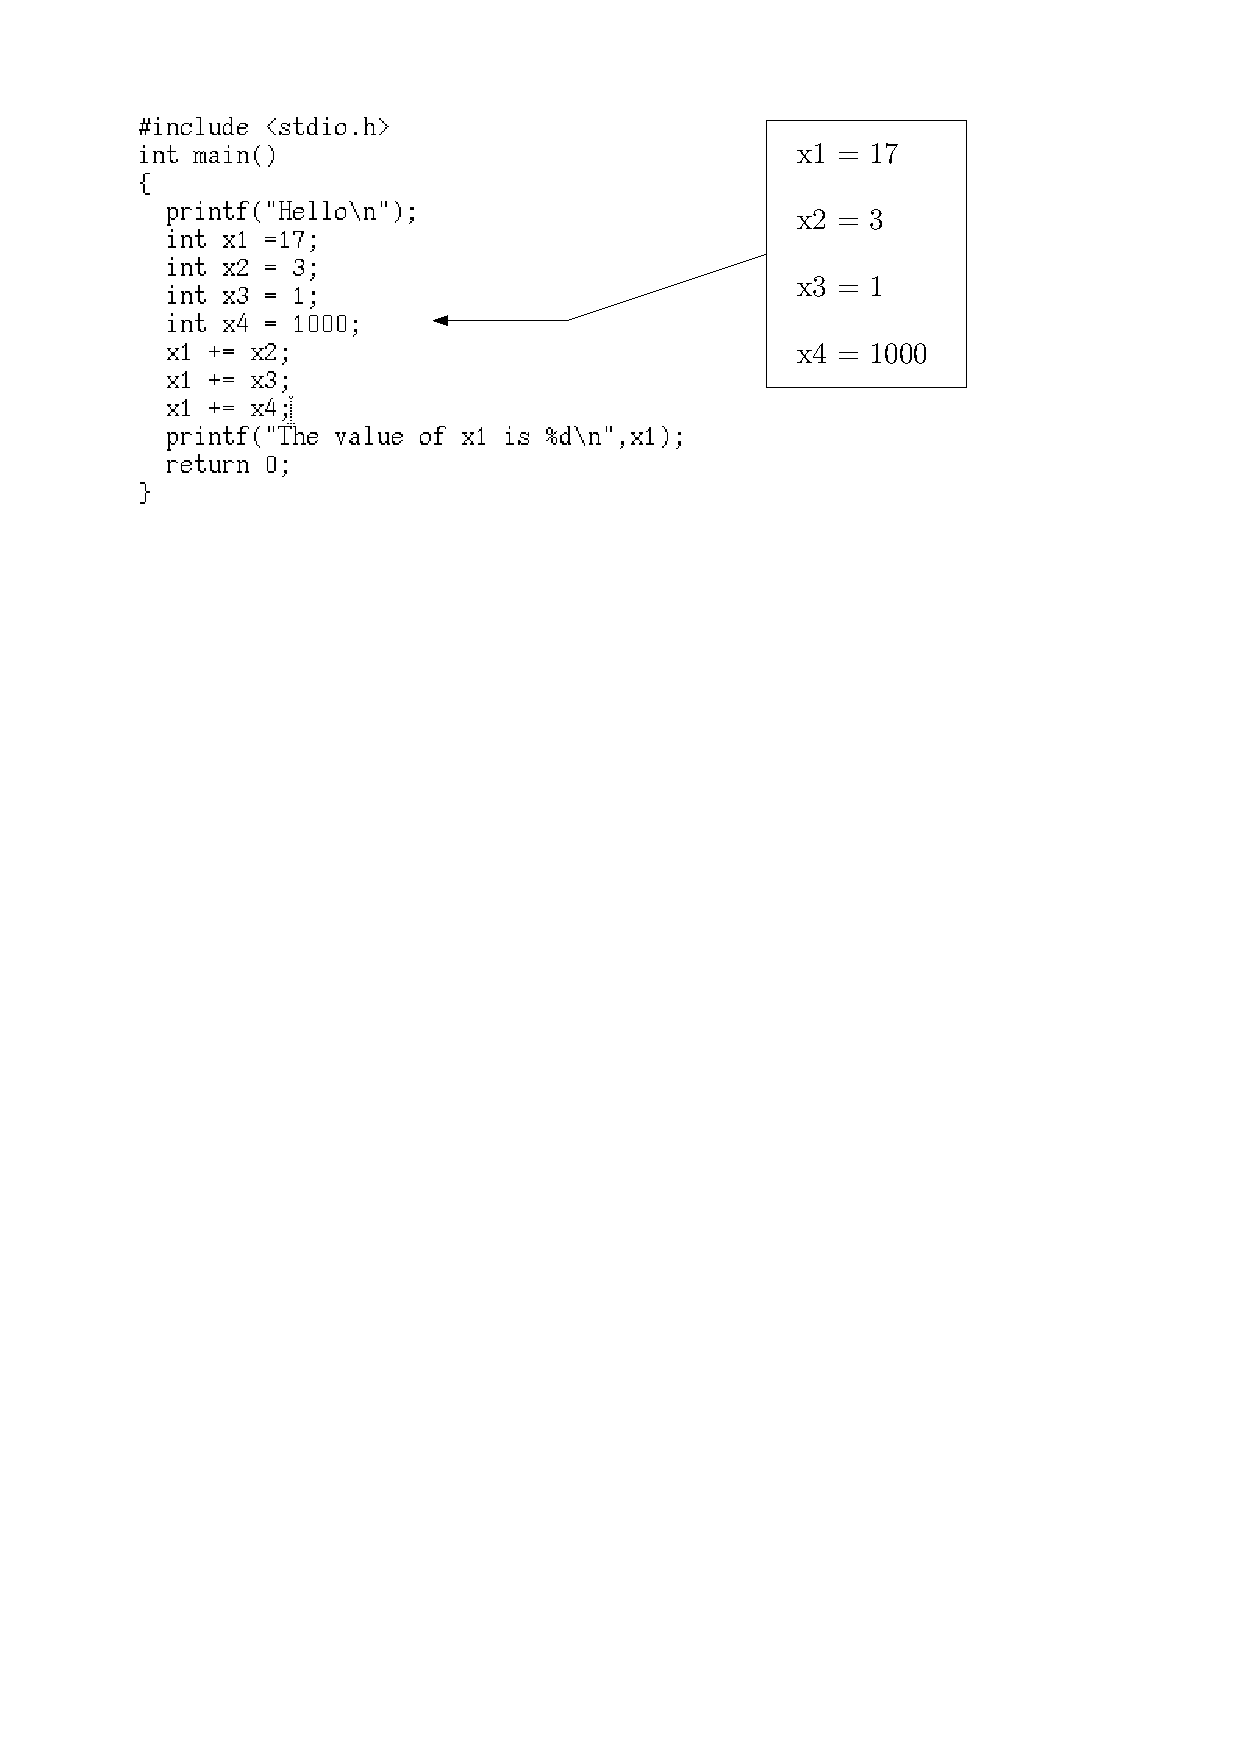
\includegraphics{model1.pdf}  \\
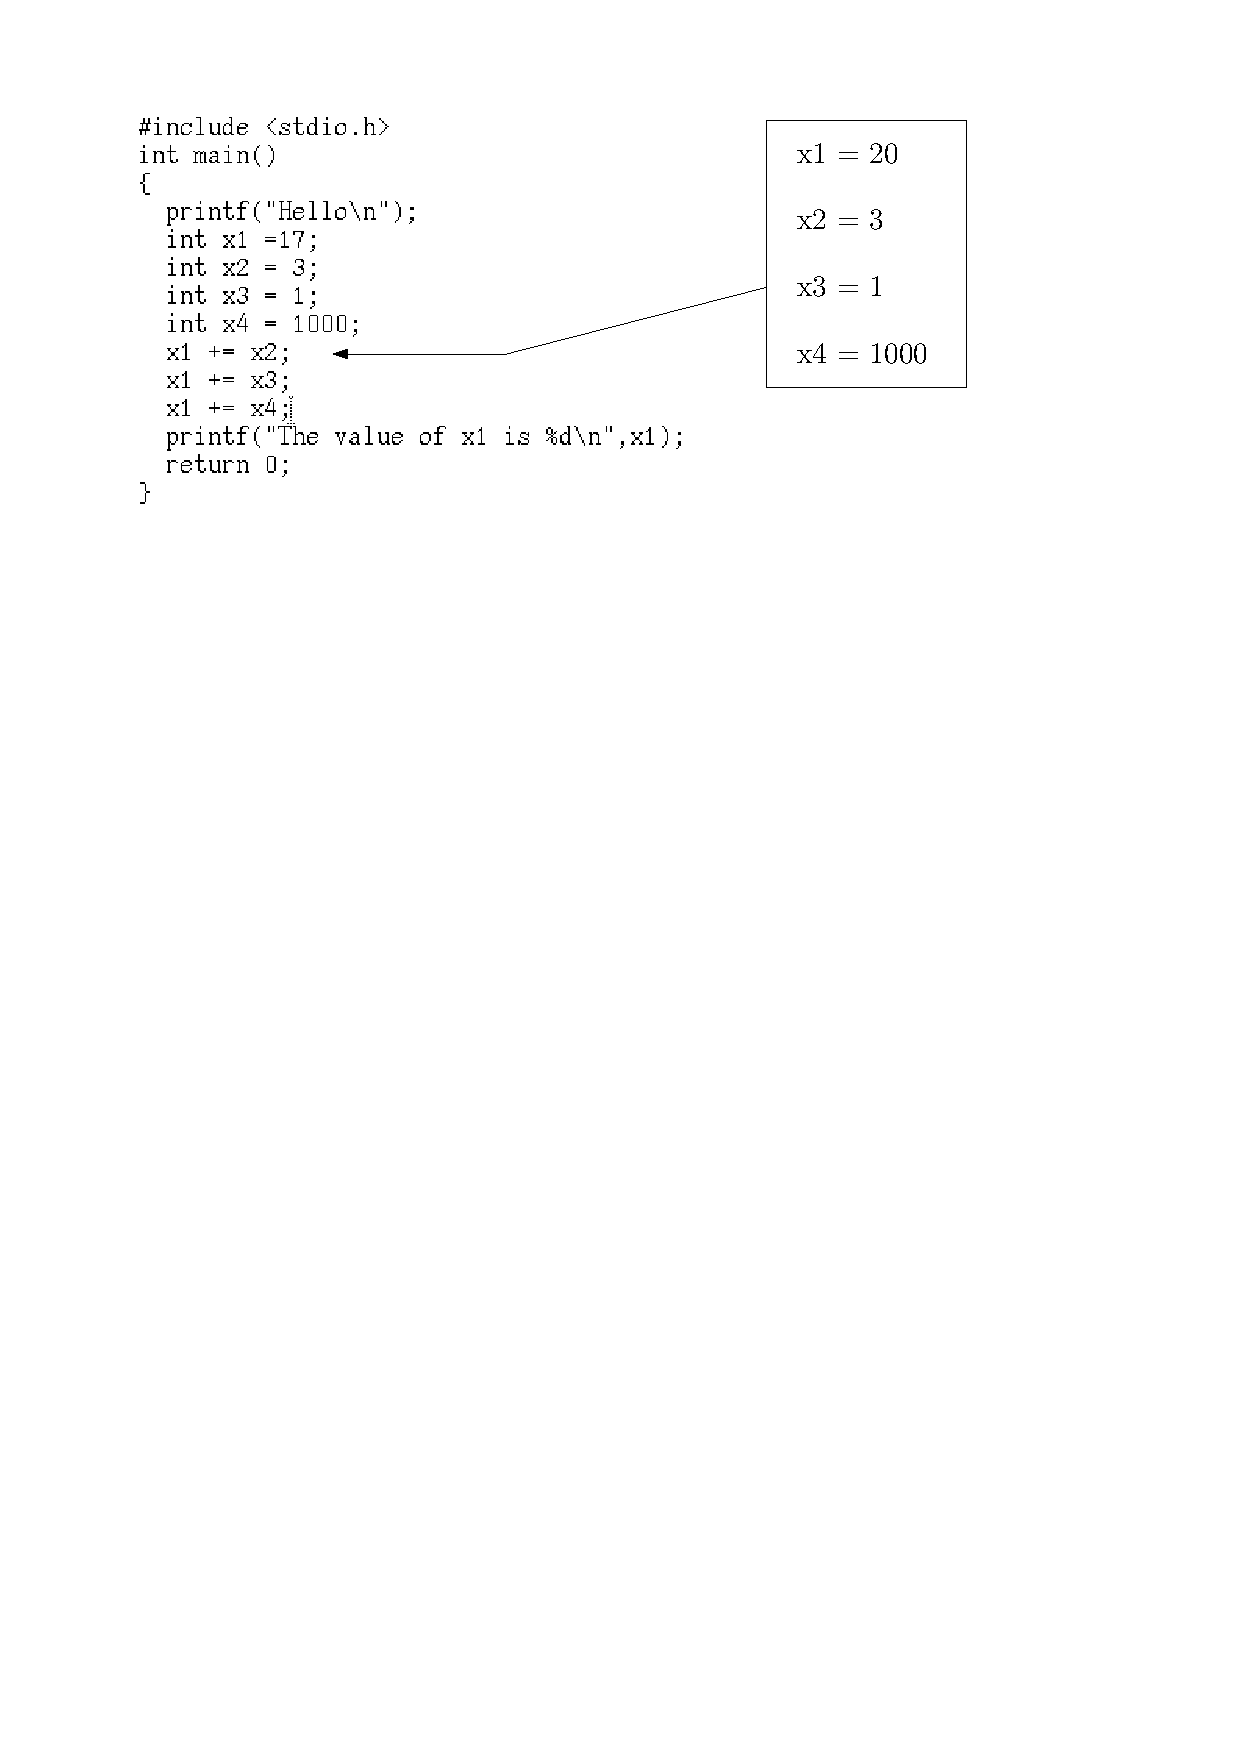
\includegraphics{model2.pdf}  \\
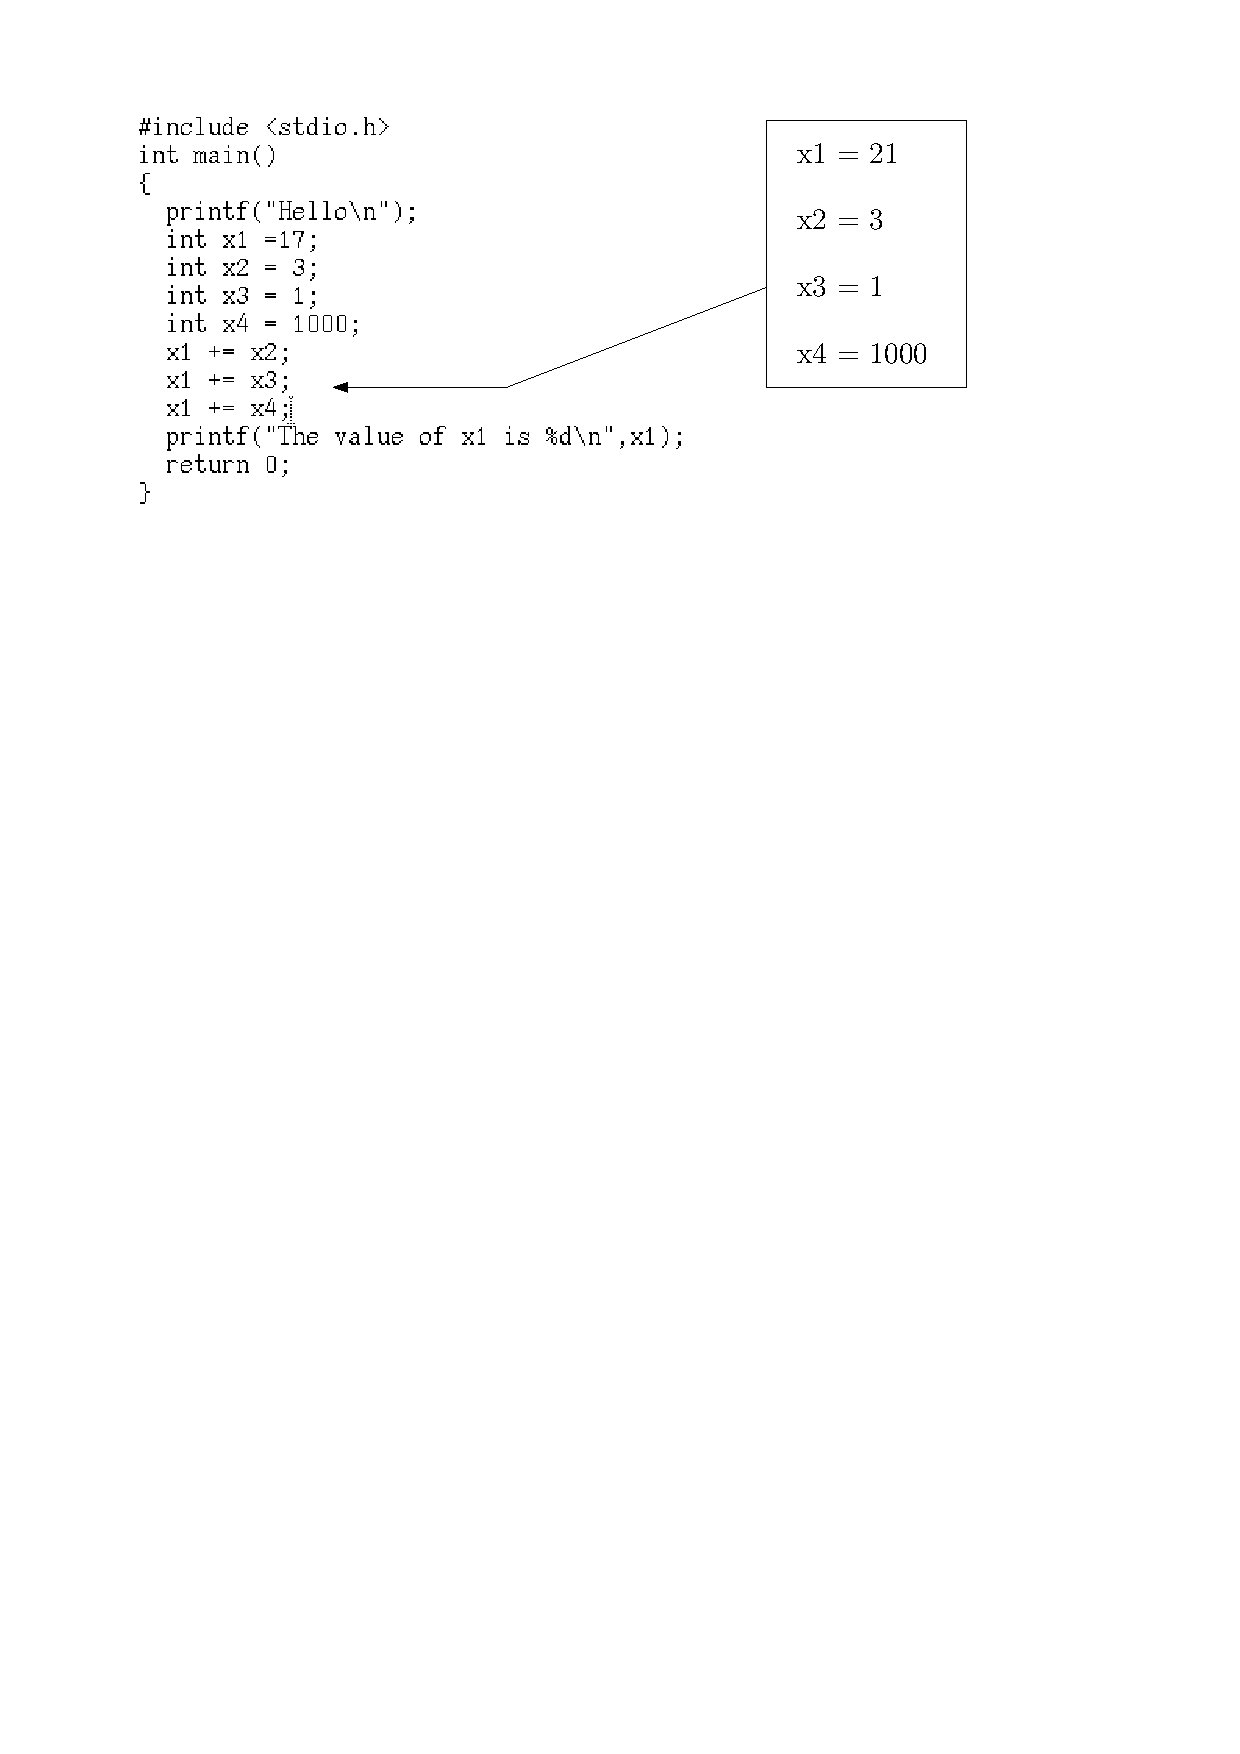
\includegraphics{model3.pdf}  \\
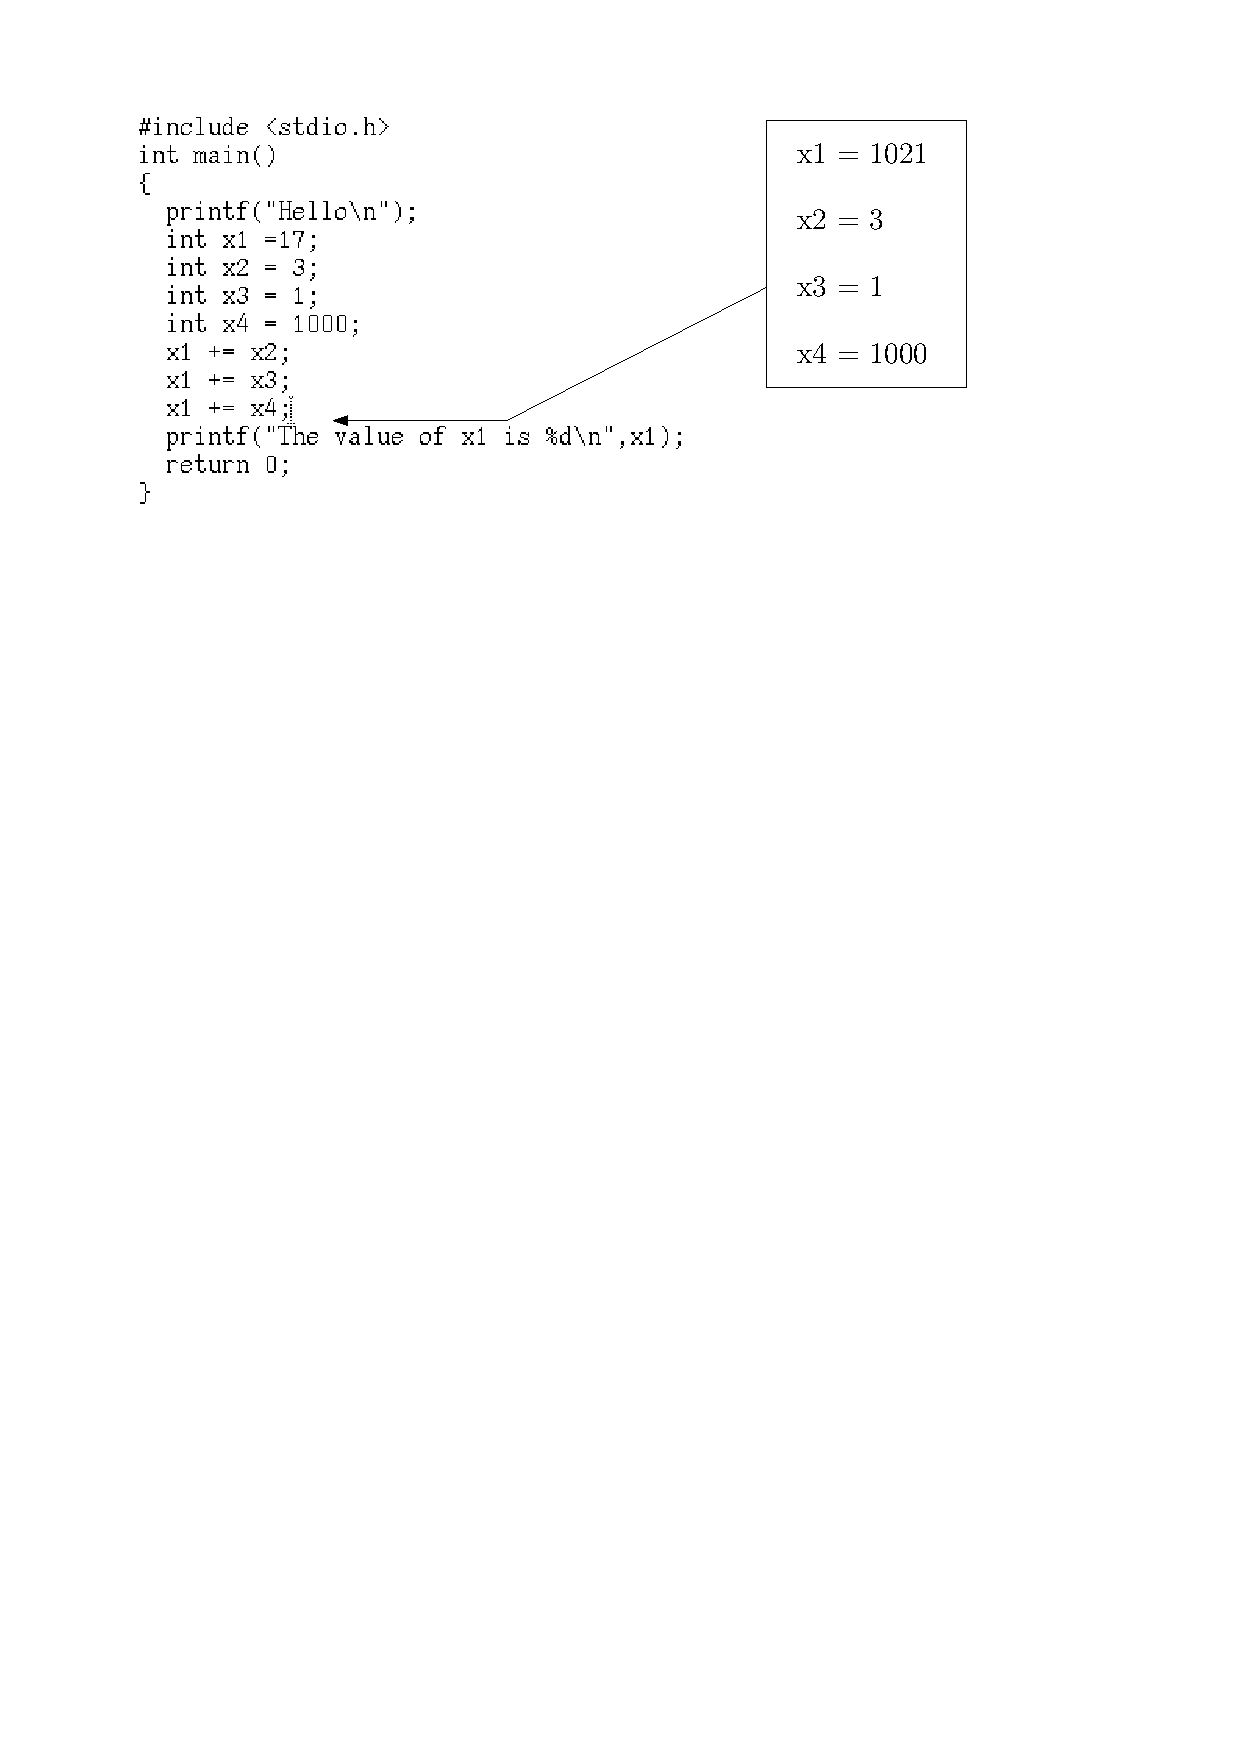
\includegraphics{model4.pdf}  \\
\clearpage
The following code is a simple ASM program to display Hello
This command is used to create the executable linking to the dynamic system libraries: \\
\verb|as -gstabs -o lab.o lab.s|
\verb|ld -dynamic-linker /lib/ld-linux.so.2 -o labasm lab.o -lc|la
\begin{GFT}{asm source code written to file lab.s}
\+.data \#Where to list any memory storage you will need for data\\
\+fmt: .string "Hello from asm\Backslash{}n"\\
\+fmt2: .string "x1 = \%d\Backslash{}n"\\
\+.text \#where the program instructions live\\
\+.globl \_start \#where program starts, same as main function in C\\
\+\_start: \#define the value of \_start label\\
\end{GFT}
Display message about program
\begin{GFT}{asm source code appended to file lab.s}
\+push \$fmt\\
\+call printf\\
\+add \$4,\%esp\\
\end{GFT}
Initialize registers to some values
\begin{GFT}{asm source code appended to file lab.s}
\+mov \$17,\%eax    \#eax = 17\\
\+mov \$3,\%ebx     \#ebx = 3\\
\+mov \$1,\%ecx     \#ecx = 1\\
\+mov \$1000,\%edx  \#edx = 1000\\
\end{GFT}
Accumulate the values into the eax register
\begin{GFT}{asm source code appended to file lab.s}
\+add \%ebx,\%eax\\
\+add \%ecx,\%eax\\
\+add \%edx,\%eax\\
\end{GFT}
Display the result
\begin{GFT}{asm source code appended to file lab.s}
\+push \%eax\\
\+push \$fmt2\\
\+call printf\\
\+add \$8,\%esp\\
\end{GFT}
Exit program by calling Linux OS command exit
\begin{GFT}{asm source code appended to file lab.s}
\+mov \$1,\%eax \#1 is the number of exit system call, require status code in \%ebx\\
\+mov \$0,\%ebx \#0 is returned to the system\\
\+int \$0x80\\
\end{GFT}
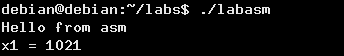
\includegraphics{labasm.png}
\end{document}
